\section{发展脉络与技术框架}
\subsection{从工具增强到研究流程组织}
科研智能体的发展并非单一路线的替代，而是知识获取、工具使用和过程组织逐步结合的结果，见图\ref{fig:timeline}。
RAG将非参数化检索与语言生成联系起来，使回答可以利用训练之外的资料\cite{rag}。
ReAct进一步通过行动获取环境观察，使检索和执行结果能够影响后续推理\cite{react}。
Toolformer则从训练角度研究模型如何决定调用何种工具、传入哪些参数以及怎样利用返回值\cite{toolformer}。
三者分别改变了信息来源、交互过程和工具调用能力，构成了科研助手进入外部环境的基础。

在此基础上，研究者开始处理长任务中的经历保留与角色协调。
Reflexion将任务反馈转化为可供后续尝试使用的文字反思\cite{reflexion}，
Generative Agents和MemGPT分别探索经历检索与分层存储\cite{generative,memgpt}。
AutoGen与MetaGPT则从代理交互、标准化交付和流程约束等角度组织多个模型实例\cite{autogen,metagpt}。
这些机制使研究活动不必在每次模型调用后重新开始，也使复杂任务可以被拆分为相互衔接的子任务。

面向科学研究的系统进一步把上述能力组合到具体场景。
ResearchAgent和SciAgents侧重利用文献关联生成研究方向，Agent Laboratory组织计算研究流程，
AI co-scientist强调候选假设的生成与演化，而Virtual Lab和Coscientist将规划与实体实验联系起来\cite{researchagent,sciagents,lab,cosci,virtual,chem}。
2026年的The AI Scientist期刊研究进一步同时讨论模板驱动和开放搜索两种模式\cite{scientistjournal}。
这些进展表明，研究焦点已由模型能否完成单个步骤，转向多个步骤如何组成可持续运行、可评价的研究过程。

\begin{figure*}[t]\centering
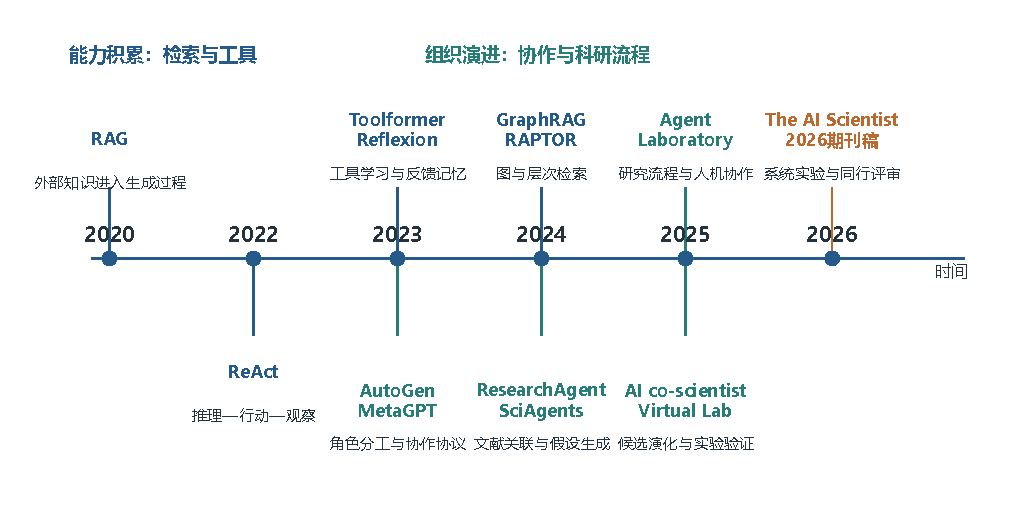
\includegraphics[width=\textwidth]{figures/review-timeline.pdf}
\caption{科研智能体相关能力与系统的代表性发展脉络。依据文献\cite{rag,react,toolformer,reflexion,autogen,metagpt,graphrag,raptor,researchagent,sciagents,lab,cosci,virtual,scientistjournal}整理。
基础工作按首次报告年份归类，2026年节点指期刊报告；时间节点为离散排布，不以间距表示持续时间。图中仅列代表工作，不表示其他路线在相应年份缺失。}
\label{fig:timeline}\end{figure*}

\subsection{科研工作流中的功能分层}
从工作流看，科研活动可以概括为问题形成、方案与实现、观察与分析、论证与交流四个相互联系的阶段。
实际研究往往在这些阶段之间往返，因而系统需要同时管理材料、状态和控制，见图\ref{fig:framework}。
知识获取负责提供外部论文、数据和工具说明；长期记忆保存项目经历及其解释；
协作控制负责选择动作、分配任务、整合输出并决定返工或停止。
三类机制分别对应信息可获得性、任务连续性与过程协调性。

这种分层有助于区分系统能力的来源。
模型没有找到相关结果，可能是检索覆盖不足；已经检索到的材料被后续阶段遗忘，涉及状态管理；
材料和状态均存在但任务仍然偏离目标，则需要检查计划与交接规则。
如果只用最终答案分数描述系统，这些性质不同的问题就容易被归入同一类“模型能力不足”。
功能分层并不要求物理上部署独立模块，而是为方法比较、系统消融和失败定位提供统一的描述方式。

\begin{figure*}[t]\centering
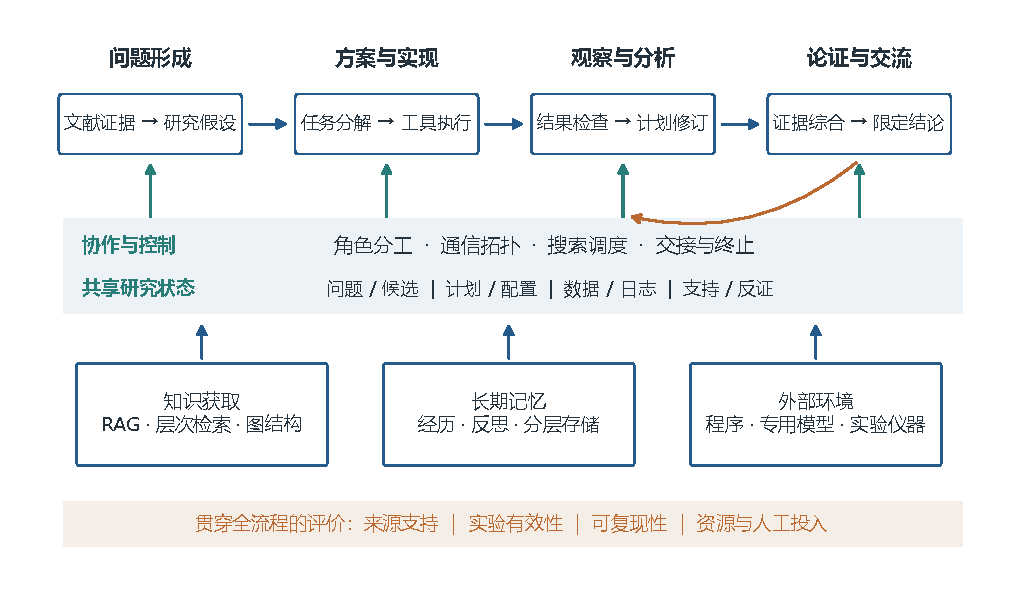
\includegraphics[width=\textwidth]{figures/review-framework.pdf}
\caption{科研工作流与支撑机制的对应关系。综合检索增强、分层记忆、代理交互与自动科研流程\cite{rag,memgpt,autogen,lab,scientistjournal}绘制。
上部为研究阶段，中部为协作及共享状态，下部为知识、记忆和环境支撑；评价贯穿整个过程。该图为综述性归纳，箭头不表示测得的效果大小。}
\label{fig:framework}\end{figure*}

\subsection{单智能体与多智能体的关系}
智能体通常由基础模型、可用工具、状态及动作选择规则共同构成。
在给定研究目标$g$下，其行为可抽象为
\begin{equation}
 a_t\sim\pi_\theta(a\mid g,o_{\leq t},m_t),
\end{equation}
其中$o_{\leq t}$为已有观察，$m_t$为当前记忆状态，$a_t$可以是检索、执行、通信或终止等动作。
该式仅用于统一描述，并不限定策略必须通过训练获得。
多智能体系统在此基础上引入不同主体之间的信息交换、任务依赖和调度规则。

因此，多智能体与单智能体之间并不存在只由数量决定的能力分界。
一个具有检索和执行反馈的代理可以完成较复杂的循环，多个代理也可能只是在重复相同推理。
多代理的实际价值取决于分解后的任务是否具有互补性、角色能否获得不同观察，以及协调开销是否小于分工收益。
本文在后续比较中将基础模型、工具能力、协作结构与计算预算分别处理，避免把系统层面的所有改进都归因于代理数量。
